\documentclass[compress,aspectratio=1610]{beamer}

\usepackage{polyglossia}
\setmainlanguage{german}
\usepackage{fontspec}
\usepackage[autostyle]{csquotes}
\usepackage{multicol}
\usepackage[percent]{overpic}
\usepackage[absolute,overlay]{textpos}
\usepackage{ulem}
\usepackage{slashed}
\usepackage{nicefrac}
\usepackage{bm}
\usepackage{siunitx}

\usetheme{vertex}

\linespread{1.1}

\title{Zeitumkehr}
\subtitle{Science~@~Sail 2019}
%\institute{Universit\"at Rostock / LHCb}
%\date{10.08.2018}
\author{Nis Meinert}

\setbeamertemplate{section page}{
    \begin{center}
		\Huge\color{vertexDarkRed}\insertsection
	\end{center}
}

\AtBeginSection{
	\begin{frame}[plain,noframenumbering]
		\sectionpage
	\end{frame}
}

\setbeamertemplate{subsection page}{
	\begin{center}
		\color{vertexDarkRed}
		\Huge\insertsection \\[10pt]
		\Large\insertsubsection
	\end{center}
}

\AtBeginSubsection{
	\begin{frame}
		\subsectionpage
	\end{frame}
}

\begin{document}

\begin{frame}[plain,noframenumbering]
    \titlepage
\end{frame}

\begin{frame}{Nis Meinert}
    \begin{columns}[T]
        \begin{column}{.6\textwidth}
            \begin{itemize}
                \item LHCb Mitglied seit 2013
                \item 2016: Master of Science (Uni. Rostock)
                \begin{itemize}
                    \item Massenspektroskopie von schweren Baryonen
                \end{itemize}
                \item Seit 2016: Doktorand am Institut für Physik (Uni. Rostock)
                \item Mehrere kürzere Aufenthalte am CERN
                \item Forschungsschwerpunkt: 
                \begin{itemize}
                    \item CP-Verletzung in Zerfällen von schweren Baryonen
                    \item Upgrade des LHCb Detektors
                \end{itemize}
            \end{itemize}
        \end{column}
        \begin{column}{.4\textwidth}
            \centering
            \begin{overpic}[height=.8\textheight,trim=200 0 0 0,clip]{img/me.png}
            \end{overpic}
        \end{column}
    \end{columns}
\end{frame}

\begin{frame}{Des Large Hadron Collider (LHC)}
    \begin{columns}[T]
        \begin{column}{.5\textwidth}
            \textbf{Der Large Hadron Collider (LHC)}
            \begin{itemize}
                \item Wikipedia: \enquote{[...] the most complex experimental facility ever built and the largest single machine in the world.}
                \item Synchrotron (in einem 27\,km langem unterirdischem Ringtunnel): \textbf{beschleunigt} u.a. Protonen auf fast Lichtgeschwindigkeit und \textbf{kollidiert} diese an bestimmten Punkten (zum Beispiel beim LHCb Detektor)
            \end{itemize}
        \end{column}
        \begin{column}{.5\textwidth}
            \centering
            \begin{overpic}[width=\textwidth]{img/cern_map.png}
            \end{overpic}
        \end{column}
    \end{columns}
\end{frame}




\begin{frame}
    \frametitle{Gliederung}
    \centering
    \scalebox{1.5}{\textbf{\textcolor{vertexDarkRed}{1.} Was ist Zeit?}}\\
    \vspace{5mm}
    \scalebox{1.5}{\textbf{\textcolor{vertexDarkRed}{2.} Makro- vs. Mikroskopische Zeit}}\\
    \vspace{5mm}
    \scalebox{1.5}{\textbf{\textcolor{vertexDarkRed}{3.} Zeitumkehr(in)varianz}}
\end{frame}

\section{Was ist Zeit?}

\begin{frame}{Was ist Zeit?}
    \begin{columns}
        \begin{column}{.65\textwidth}
            \textbf{Aristoteles} (300 BC.)
            \begin{quote}
                Die Zeit ist nichts Seiendes.
                Sie ist die \textbf{Wahrnehmung} des Davor und Danach an der \textbf{Bewegung}.
            \end{quote}
        \end{column}
        \begin{column}{.35\textwidth}
            \centering
            \includegraphics[height=.35\textheight]{img/aristoteles.png}\\
            \centering
            \scalebox{.4}{(After Lysippos [CC BY-SA 2.5])}
        \end{column}
    \end{columns}
    \begin{columns}
        \begin{column}{.35\textwidth}
            \centering
            \includegraphics[height=.35\textheight]{img/newton.png}\\
            \centering
            \scalebox{.4}{(After Godfrey Kneller [Public domain])}
        \end{column}
        \begin{column}{.65\textwidth}
            \textbf{Newton} (1700 AD.)
            \begin{quote}
                Die absolute, wahre und mathematische Zeit fließt an sich und ihrer Natur nach gleichmäßig, \textbf{ohne Beziehung auf äußere Gegenstände}.
                (Insbesondere \textbf{unabhängig von einem Beobachter}.)
            \end{quote}
        \end{column}
    \end{columns}
\end{frame}

\begin{frame}{Was ist Zeit?}
    \begin{columns}
        \begin{column}{.55\textwidth}
            \textbf{2. Newtonsche Gesetz}
            \begin{quote}
            Um einen Körper (Masse $m$) zu beschleunigen ($v(t_1) \to v(t_2)$) braucht man Kraft $F$!
            \end{quote}

            \begin{equation*}
                F(t) \approx m \cdot \underbrace{\frac{v(t_2) - v(t_1)}{t_2 - t_1}}_{\text{Ableitung}}
            \end{equation*}
        \end{column}
        \begin{column}{.45\textwidth}
            \centering
            \includegraphics{img/taxis.png}\\
        \end{column}
    \end{columns}

    \centering
    In \textbf{Bewegungsgleichungen} verknüpfen Ableitungen Zeitpunkt $t$ mit \textbf{Vergangenheit} ($t_1$) und \textbf{Zukunft} ($t_2$)!
\end{frame}

\begin{frame}{Was ist Zeit?}
    \begin{columns}
        \begin{column}{.35\textwidth}
            \centering
            \includegraphics[height=.35\textheight]{img/newton.png}\\
            \centering
            \scalebox{.4}{(After Godfrey Kneller [Public domain])}
        \end{column}
        \begin{column}{.65\textwidth}
            \textbf{Newton}\\
            Physik beschreibt Natur im Raum (3D) und \textbf{unabhängig} davon in der absoluten Zeit.
        \end{column}
    \end{columns}
    \begin{columns}
        \begin{column}{.65\textwidth}
            \textbf{Einstein}\\
            Physik beschreibt Natur in \textbf{vier}dimensionaler Raumzeit.
            \begin{itemize}
                \item Zeit vergeht an verschiedenen Orten unterschiedlich schnell
            \end{itemize}
        \end{column}
        \begin{column}{.35\textwidth}
            \centering
            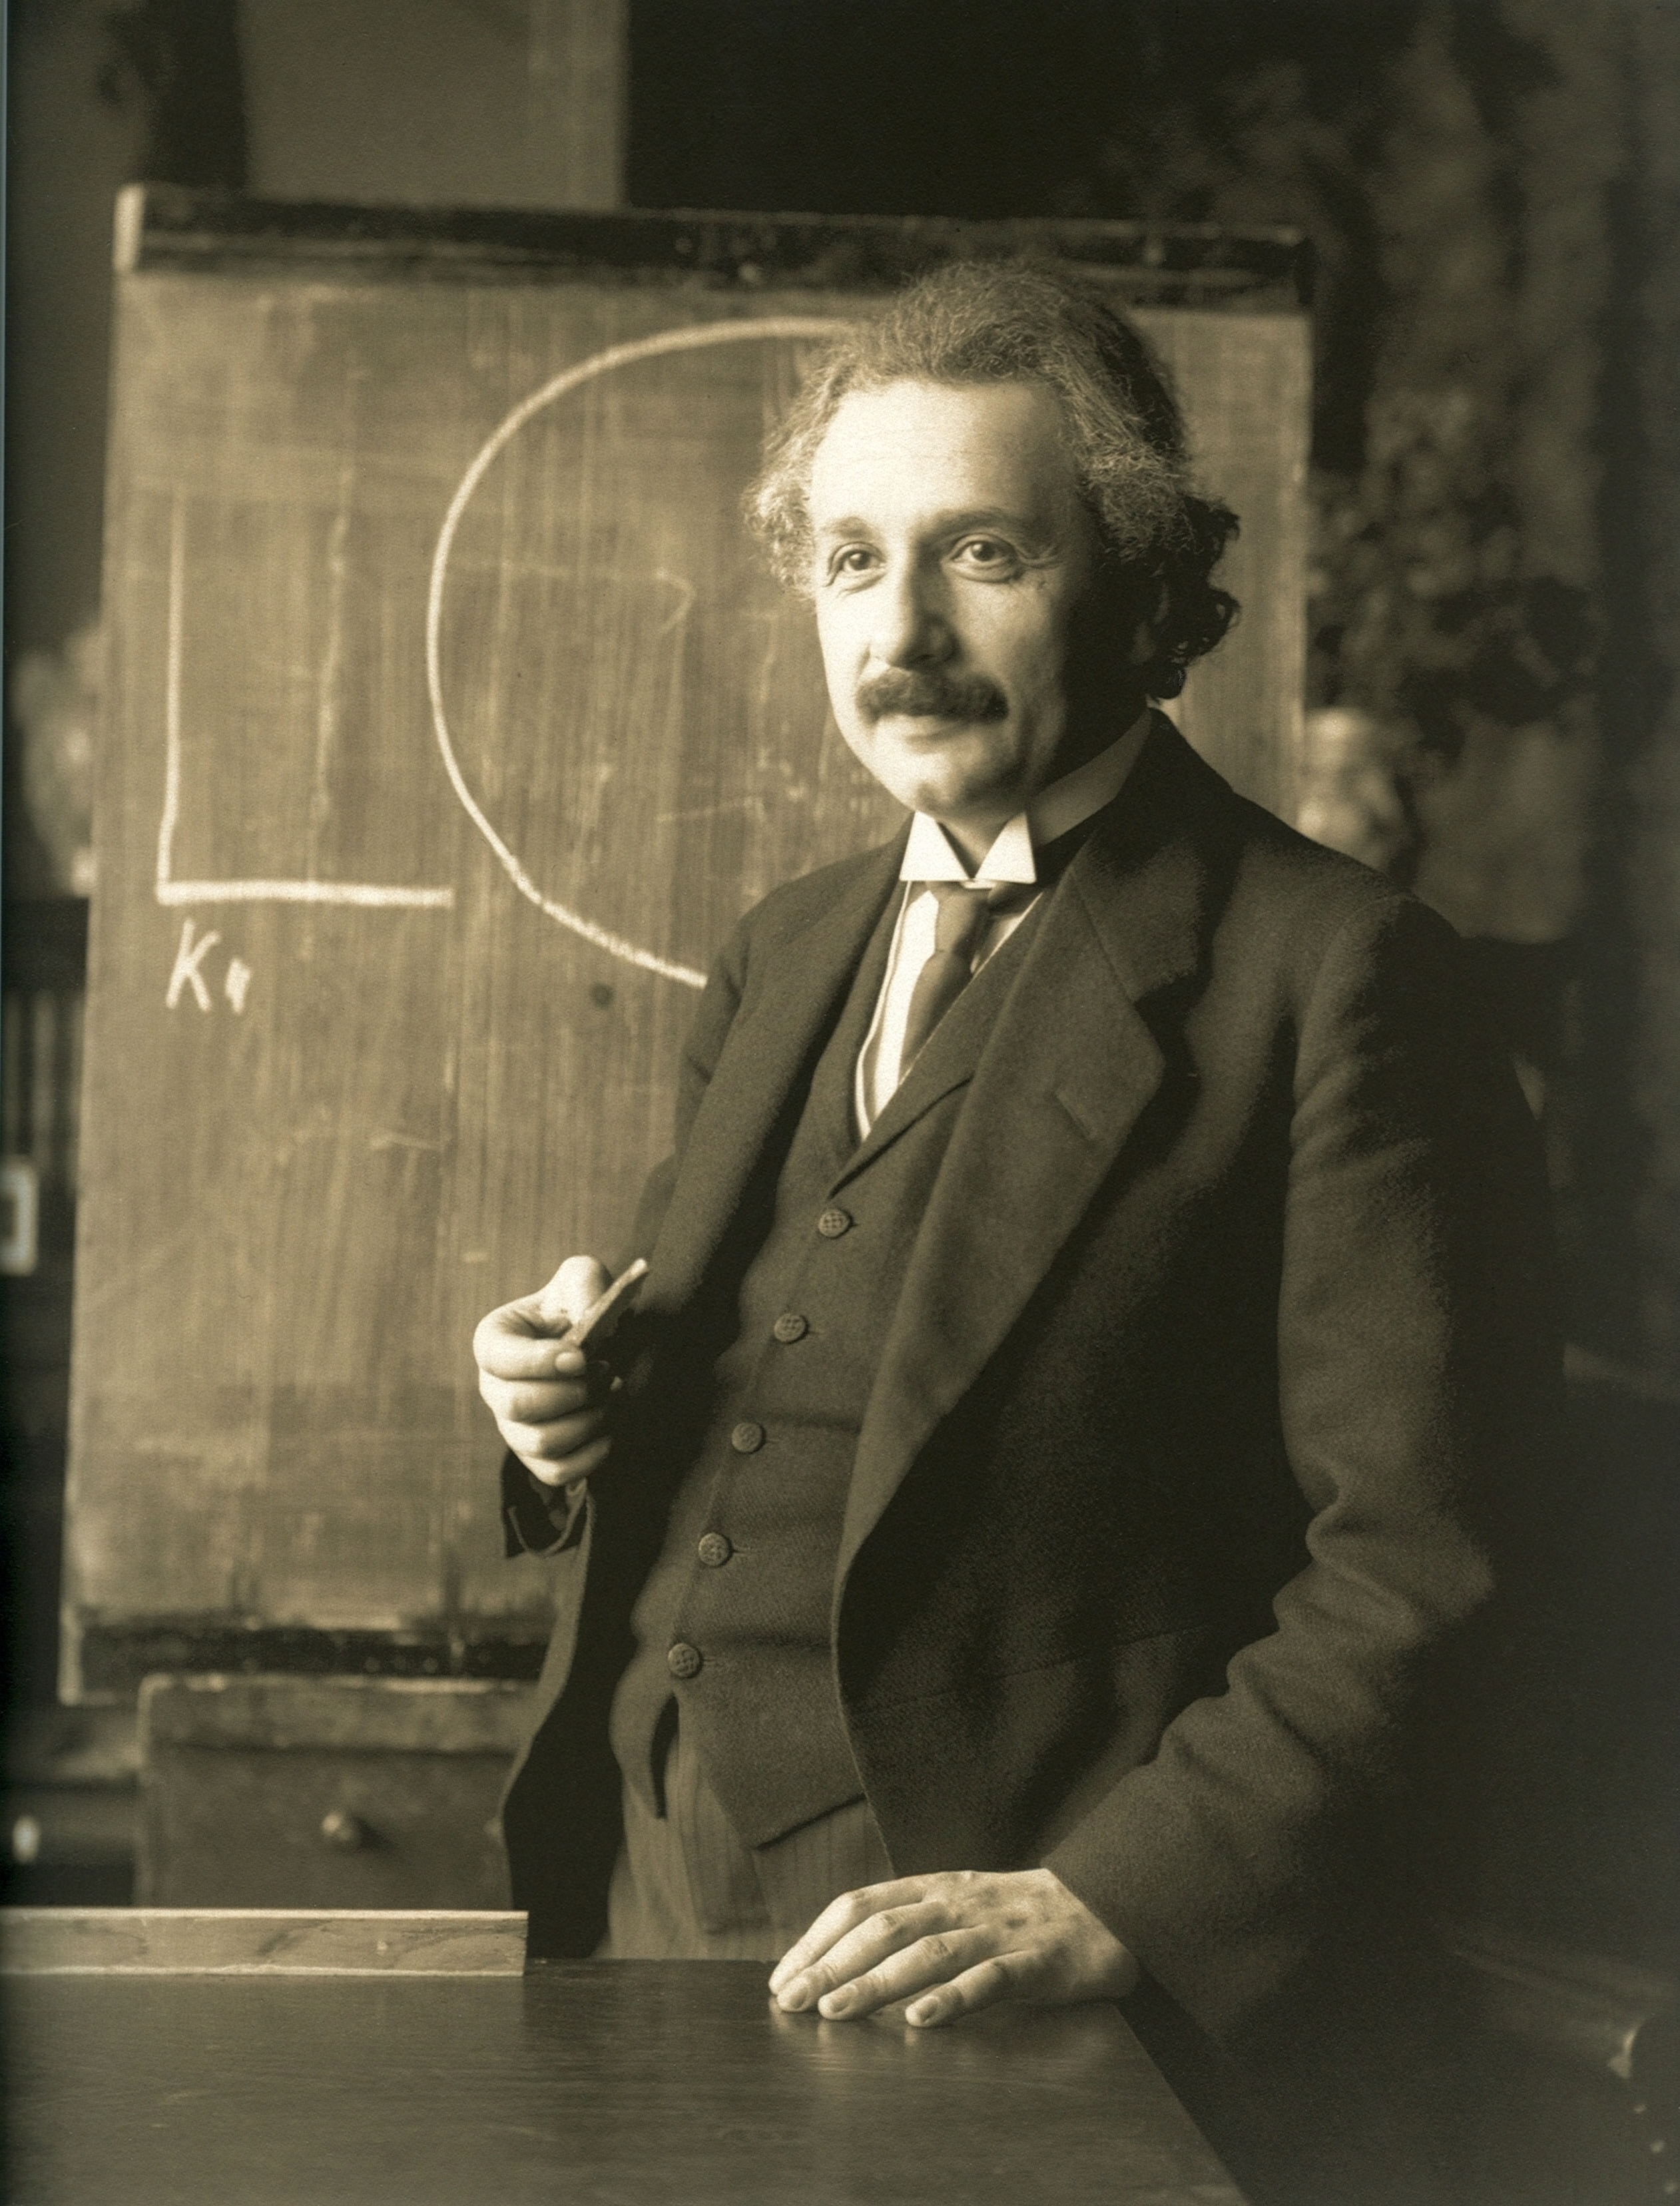
\includegraphics[height=.35\textheight]{img/einstein.png}\\
            \centering
            \scalebox{.4}{(Ferdinand Schmutzer [Public domain])}
        \end{column}
    \end{columns}
\end{frame}

\begin{frame}{Was ist Zeit?}
    \begin{columns}
        \begin{column}{.6\textwidth}
            \textbf{(Spezielle) Relativitätstheorie}\\
            \begin{itemize}
                \item In Bewegung vergeht die Zeit langsamer (Zwillingsparadoxon!)
                \item Gleichzeitigkeit ist subjektiv
                \item \textbf{Aber:} Kausalität bleibt stets gewahrt! (untere Grenzen für Zeitreisen)
            \end{itemize}
        \end{column}
        \begin{column}{.4\textwidth}
            \centering
            \includegraphics[height=.35\textheight]{img/cascade.png}\\
            \centering
            \scalebox{.4}{(aussiegall [CC BY 2.0])}
        \end{column}
    \end{columns}
\end{frame}

\begin{frame}{Was ist Zeit?}
    \begin{columns}
        \begin{column}{.65\textwidth}
            \textbf{Relativitätstheorie}\\
            \begin{itemize}
                \item Zeit vergeht an verschiedenen Orten unterschiedlich schnell
                \item Es gibt keine globale Gleichzeitigkeit
                \item Kausalität ist eine invariante und gilt in allen Bezugssystemen gleichermaßen
            \end{itemize}
        \end{column}
        \begin{column}{.35\textwidth}
            \centering
            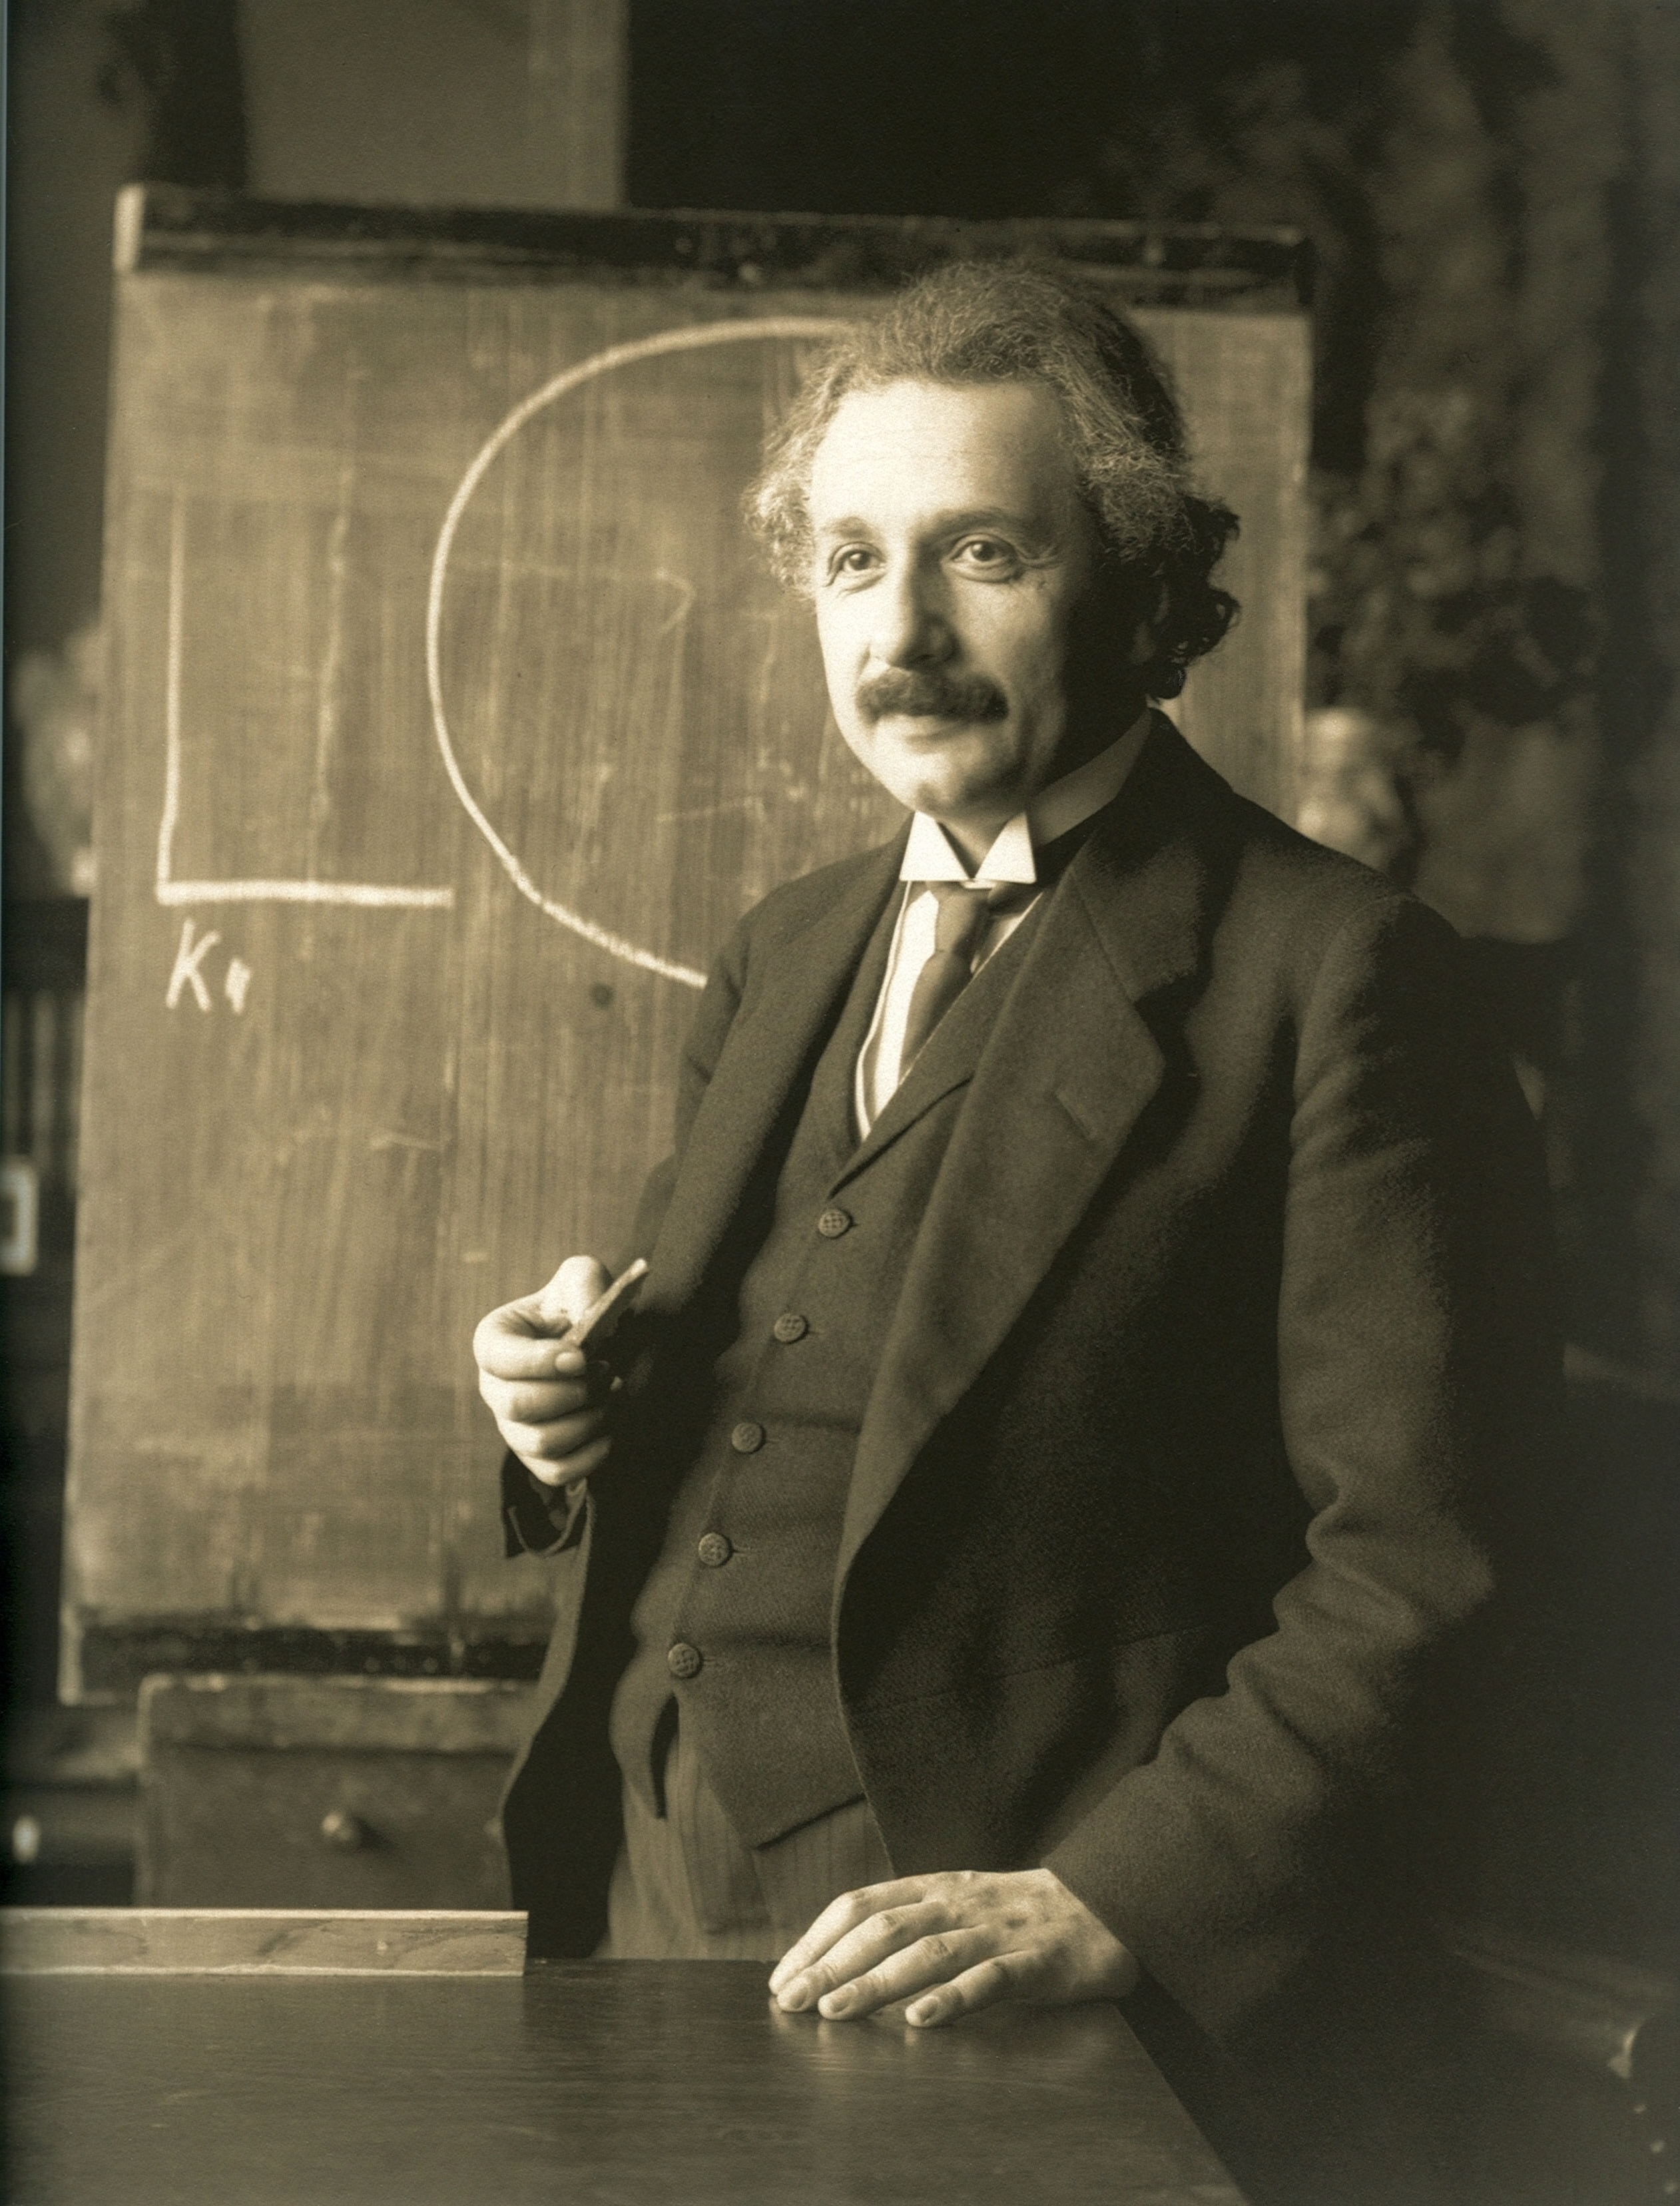
\includegraphics[height=.35\textheight]{img/einstein.png}\\
            \centering
            \scalebox{.4}{(Ferdinand Schmutzer [Public domain])}
        \end{column}
    \end{columns}

    \begin{center}
        \scalebox{2.}{\&}
    \end{center}

    \textbf{Quantenphysik:} Materie und Raumzeit sind untrennbar (es gibt keinen leeren Raum!)
    \begin{center}
        $\Delta E \cdot \Delta t \ge \hbar / 2$
    \end{center}
\end{frame}

\section{Makro- vs. Mikroskopische Zeit}

\begin{frame}{Staubsimulation}
    \begin{columns}
        \begin{column}{.6\textwidth}
            \textbf{Einfache Staubsimulation}
            \begin{itemize}
                \item Zu Beginn: 25 Staubkörner, in der Mitte des Raumes
                \item Jedes Staubkorn kann sich zufällig in eine beliebige Richtung bewegen
                \item \textbf{Aufgabe}: Bilder zeitlich ordnen!
            \end{itemize}

            \only<2>{%
            \begin{center}
                \scalebox{2.}{$\downarrow$}

                \vspace{5mm}
                Ist das Zeit?
            \end{center}}
        \end{column}
        \begin{column}{.2\textwidth}
            \begin{figure}
                \includegraphics{img/dust_init}
                \caption{$t = 0\,$h}
            \end{figure}
            \begin{figure}
                \includegraphics{img/dust_t2}
                \caption{\only<1>{$t=$???}\only<2>{$t=2\,$h}}
            \end{figure}
        \end{column}
        \begin{column}{.2\textwidth}
            \begin{figure}
                \includegraphics{img/dust_t1}
                \caption{\only<1>{$t=$???}\only<2>{$t=1\,$h}}
            \end{figure}
            \begin{figure}
                \includegraphics{img/dust_t3}
                \caption{\only<1>{$t=$???}\only<2>{$t=4\,$h}}
            \end{figure}
        \end{column}
    \end{columns}
\end{frame}

\begin{frame}{Staubsimulation}
    \centering
    \textbf{Welcher Zustand ist nach 4\,h wahrscheinlicher?}

    \vspace{5mm}
    \includegraphics{img/dust_t3} 
    \hspace{5mm} 
    \includegraphics{img/dust_fake} 

    \vspace{5mm}
    \only<2>{Beide Zustände sind gleich wahrscheinlich!}
\end{frame}

\begin{frame}{Entropie}
    \begin{columns}
        \begin{column}{.7\textwidth}
            \textbf{Welcher Zustand ist nach 4\,h wahrscheinlicher?}
            \begin{itemize}
                \item (a) und (b) sind \textbf{gleich wahrscheinlich} \ldots
                \item \ldots aber es gibt viel mehr Konfigurationen die (a) ähnlicher sehen als (b)
            \end{itemize}
            \begin{center}
                \scalebox{2.}{$\downarrow$}

                \vspace{5mm}
                \textbf{Makroskopische Zeit:} Übergang in einen wahrscheinlicheren Zustand (\textbf{Entropie})
            \end{center}
        \end{column}
        \begin{column}{.3\textwidth}
            \centering
            \begin{figure}
                \includegraphics{img/dust_t3}
                \caption{(a)}
            \end{figure}

            \begin{figure}
                \includegraphics{img/dust_fake}
                \caption{(b)}
            \end{figure}
        \end{column}
    \end{columns}
\end{frame}

\begin{frame}{Entropie}
    \begin{columns}
        \begin{column}{.7\textwidth}
            \textbf{Entropiezunahme}
            \begin{itemize}
                \item Physik: Entropie nimmt (global) immer zu 
                \item Seit dem Urknall entwickeln wir uns also in immer wahrscheinlichere Klassen von Zuständen (\textit{morgen ist wahrscheinlicher als gestern}) \ldots
                \item \ldots ähnlich wie Staub in unserer Wohnung
                \item<2> Dieser Prozess ist \textbf{rein statistisch und würde auch zeitgespiegelt genauso ablaufen!}
            \end{itemize}
        \end{column}
        \begin{column}{.3\textwidth}
            \centering
            \includegraphics{img/dust_init}

            \vspace{5mm}
            \scalebox{2.}{$\downarrow$}

            \vspace{5mm}
            \includegraphics{img/dust_t3}
        \end{column}
    \end{columns}
\end{frame}

\begin{frame}{Makro- vs. Mikroskopische Zeit}
    \begin{columns}
        \begin{column}{.6\textwidth}
            \textbf{Makro- vs. Mikroskopische Zeit}
            \begin{itemize}
                \item Makroskopisch: Entropie oktroyiert Richtung des Zeitflusses (Statistik)
                \begin{itemize}
                    \item Entwicklung zur wahrscheinlichsten Zustandsklasse
                \end{itemize}
                \item Mikroskopisch: Zeitentwicklung innerhalb einer Zustandsklasse mit gleicher Entropie (physikalische Zeit $t$)
            \end{itemize}
        \end{column}
        \begin{column}{.4\textwidth}
            \centering
            \includegraphics[width=\textwidth]{img/dali.png}\\
            \scalebox{.4}{(Low resolution: Salvador Dal\'i 1931 \textit{The Persistence of Memory})}
        \end{column}
    \end{columns}
\end{frame}

\begin{frame}{Physikalische Zeit $t$ (Mikroskopische Zeit)}
    \begin{columns}
        \begin{column}{.6\textwidth}
            \textbf{Beispiel: Steinwurf}
            \begin{itemize}
                \item Werfe Stein mit $36\,$km/h in die Luft
                \item Stein fliegt $1\,$s hoch
                \item $1\,$s runter
                \item und landet mit $36\,$km/h
            \end{itemize}

            \centering
            \vspace{5mm}
            \textbf{Dieser Prozess ist Zeitsymmetrisch!${}^{\color{vertexDarkRed}\star}$}

            \scalebox{.7}{${}^{\color{vertexDarkRed}\star}$ sofern der Stein einen Grund findet von alleine abzuheben ($\rightarrow$ Entropie)}
        \end{column}
        \begin{column}{.4\textwidth}
            \centering
            \includegraphics[width=\textwidth]{img/toss}
        \end{column}
    \end{columns}

    \centering
    \vspace{5mm}
    \scalebox{1.5}{\only<2>{Sind alle physikalischen Prozesse zeitsymmetrisch?}\vphantom{Foobar}}
\end{frame}

\begin{frame}{Zeitsymmetrie}
    \centering
    \scalebox{1.5}{Sind alle physikalischen Prozesse zeitsymmetrisch?}

    Antwort bis 1963: \textbf{ja!}
\end{frame}

\begin{frame}{Physik im Jahre 1963}
    \begin{columns}
        \begin{column}{.6\textwidth}
            \textbf{CPT Theorem (gilt bis heute!)}
            \begin{itemize}
                \item Jede physikalische Theorie ist invariant unter
                \begin{itemize}
                    \item Raumspiegelung \&
                    \item Ladungsspiegelung \&
                    \item Zeitumkehr
                \end{itemize}
                \item Seit 1957: Natur ist \textbf{nicht} invariant unter (alleiniger) Raumspiegelung
                \begin{itemize}
                    \item Wu-Experiment: Radioaktive Kernzerfälle erscheinen im Spiegel unphysikalisch
                    \item Invarianz wird wieder hergestellt durch zusätzliche Ladungsspiegelung
                \end{itemize}
            \end{itemize}
        \end{column}

        \begin{column}{.4\textwidth}
            \centering
            \includegraphics[height=.7\textheight]{img/wu}
            \scalebox{.4}{(Wu Experiment [Public domain])}
        \end{column}
    \end{columns}

    \vspace{5mm}
    \centering
    Ist unser Universum invariant unter Raum- \& Ladungsspiegelung $\Leftrightarrow$ Zeitumkehr?
\end{frame}

\begin{frame}{Einschub: Antimaterie und Spiegelwelten}
    \begin{columns}
        \begin{column}{.7\textwidth}
            \textbf{Antimaterie und Spiegelwelten} 
            \begin{itemize}
                \item Zu jedem Materie Baustein existiert ein dazugehöriger Antimaterie Baustein
                \item Zusammenhang Materie \& Antimaterie: Ladungsspiegelung (das \enquote{C} in CPT)
                \only<1>{%
                \item Wu Experiment zeigt:
                \begin{itemize}
                    \item Schwache Kernzerfälle unterscheiden fundamental zwischen Ladung
                    \item Unterscheidung wird kompensiert durch Raumspiegelung (das \enquote{P} in CPT)
                    \item \textbf{Wu-Experiment ist invariant unter Raum- \& Ladungsspiegelung} (CP)
                \end{itemize}}%
                \only<2>{%
                \item Makroskopisch sind alle Zustände ladungsneutral:
                \begin{itemize}
                    \item Antimaterie verhält sich wie räumlich gespiegelte Materie
                    \item CPT: Antimaterie verhält sich wie zeitlich rückwärts laufende Materie
                    \item \textbf{\textit{im Spiegel läuft die Zeit rückwärts}}${}^{\color{vertexDarkRed}\star}$ (Entropie lässt uns altern)
                \end{itemize}
                \scalebox{.5}{${}^{\color{vertexDarkRed}\star}$ Korrekt\textit{er}: Das Spiegelbild verhält sich wie ein (ladungsneutrales) Universum mit gespiegelter (mikroskopischer) Zeit}}
            \end{itemize}
        \end{column}
        \begin{column}{.3\textwidth}
            \centering
            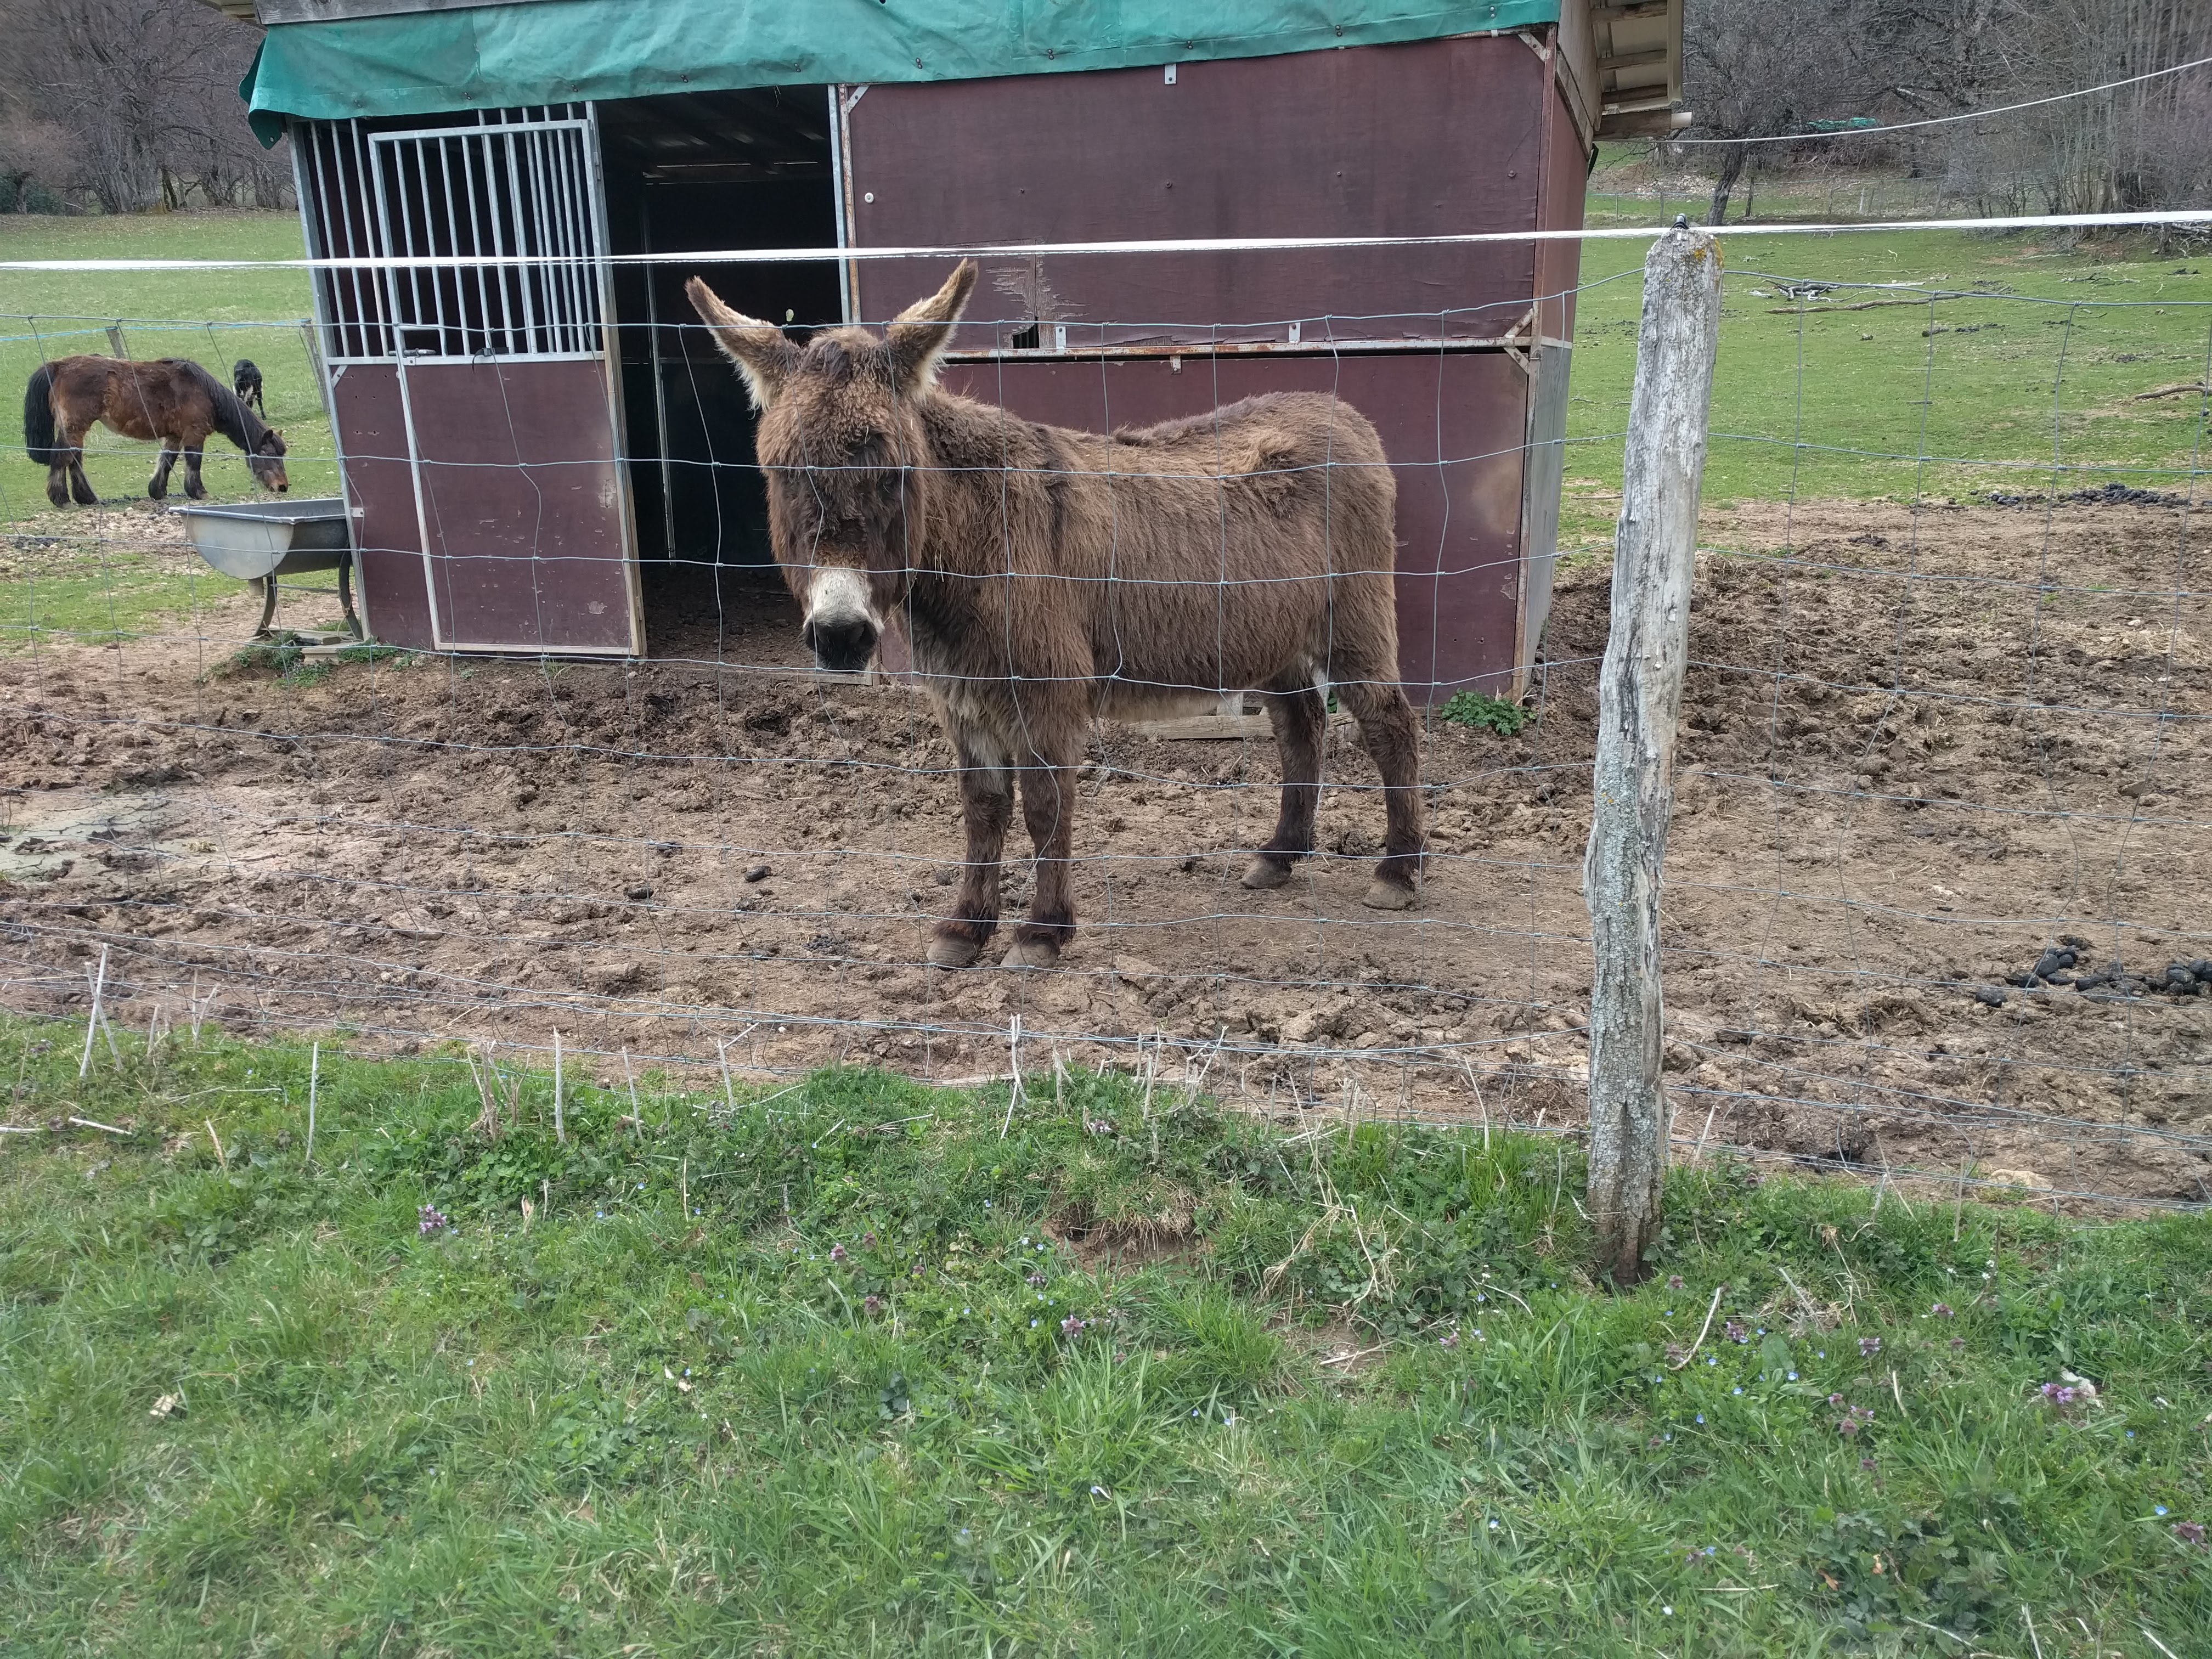
\includegraphics[height=.25\textheight]{img/donkey}\\
            \scalebox{.8}{Esel}

            \vspace{5mm}
            \scalebox{2.}{$\updownarrow$}

            \vspace{5mm}
            \includegraphics[height=.25\textheight]{img/anti_donkey}\\
            \scalebox{.8}{Anti-Esel}
        \end{column}
    \end{columns}
\end{frame}

\begin{frame}{Zeitumkehrsymmetrie: Implikationen}  
    \scalebox{1.5}{Ist unser Universum invariant unter}
    \scalebox{1.5}{Raum- \& Ladungsspiegelung $\Leftrightarrow$ Zeitumkehr?}
    \begin{itemize}
        \item Definition von Materie und Antimaterie willkürlich?
        \begin{itemize}
            \item Würden wir es bemerken, wenn über Nacht alle Materie zu Antimaterie wird?
        \end{itemize}
        \item Definition der Zeitrichtung willkürlich? 
        \begin{itemize}
            \item Würden wir es bemerken, wenn sich über Nacht die Zeit umkehrt?
        \end{itemize}
    \end{itemize}

    Antwort bis 1963: \textbf{nein!}
\end{frame}

\begin{frame}{Zeitumkehrsymmetrie}  
    \begin{columns}
        \begin{column}{.6\textwidth}
            \textbf{Experimentelle Herausforderung}
            \begin{itemize}
                \item Raum-, Ladungs- und Zeitspiegelungen sind diskrete Transformationen
                \begin{itemize}
                    \item ein Experiment kann nicht langsam und kontinuierlich in sein Spiegelbild überführt werden
                \end{itemize}
                \item Ansatz Wu-Experiment (Raumspiegelung)
                \begin{enumerate}
                    \item experimenteller Aufbau im Labor
                    \item betrachte Aufbau im Spiegel
                    \item baue Spiegelbild nach
                    \item vergleiche (2.) und (3.)
                \end{enumerate}
                \item Zeitspiegelung?
            \end{itemize}
        \end{column}

        \begin{column}{.4\textwidth}
            \centering
            \includegraphics[height=.7\textheight]{img/wu}
            \scalebox{.4}{(Wu Experiment [Public domain])}
        \end{column}
    \end{columns}
\end{frame}

\begin{frame}{1964: Beobachtung von CP Verletzung}  
    \begin{columns}
        \begin{column}{.7\textwidth}
            \begin{itemize}
                \item James Cronin und Val Fitch (Brookhaven) entdecken, dass sich das Materieteilchen $K^0$ und sein Antiteilchen $\bar K^0$ in Zerfällen unterschiedlich verhalten
                \item Materie und Antimaterie lassen sich damit \textbf{eindeutig} definieren
                \item Nobelpreis: 1980
                \item Schlußfolgerung CPT: Zeitumkehr ist (auch) keine Invariante!
            \end{itemize}
        \end{column}

        \begin{column}{.3\textwidth}
            \centering
            \includegraphics[width=\textwidth]{img/nobelprize}
            \scalebox{.4}{(Noble Prize [Public domain])}
        \end{column}
    \end{columns}
\end{frame}

\begin{frame}{Direkter Nachweis von Zeitsymmetrie Verletzung}
    \begin{columns}
        \begin{column}{.7\textwidth}
            \textbf{Oszillation}
            \begin{itemize}
                \item Manche Teilchen können in ihr eigenes Antiteilchen oszillieren, z.B $K^0 \!\leftrightarrow \bar K^0$
                \item $K^0$ (Teilchen) wandelt sich sporadisch in $\bar K^0$ (Antiteilchen) und umgekehrt
                \item Wenn Symmetrie zwischen Materie und Antimaterie perfekt
                \begin{itemize}
                    \item $K^0 \!\to \bar K^0$ genauso häufig wie $\bar K^0 \!\to K^0$
                \end{itemize}
                \item Alternativ: Wenn Zeitumkehrsymmetrie perfekt
                \begin{itemize}
                    \item $K^0 \!\to \bar K^0$ genauso häufig wie $K^0 \!\leftarrow \bar K^0$
                \end{itemize}
            \end{itemize}
        \end{column}

        \begin{column}{.3\textwidth}
            \centering
            \includegraphics[width=\textwidth]{img/kafka}
        \end{column}
    \end{columns}
\end{frame}

\begin{frame}{Direkter Nachweis von Zeitsymmetrie Verletzung}
    \begin{columns}
        \begin{column}{.6\textwidth}
            \textbf{CPLEAR Experiment} (CERN)
            \begin{itemize}
                \item Betrachtet symmetrische $K^0$ und $\bar K^0$ Produktion (in $p \bar p$ Kollisionen)
                \item Zählt (zeitaufgelöst) Anzahlen
                \begin{itemize}
                    \item $N(K^0 \!\to \bar K^0)$
                    \item $N(\bar K^0 \!\to K^0)$
                \end{itemize}
            \end{itemize}
        \end{column}

        \begin{column}{.4\textwidth}
            \centering
            \includegraphics[width=\textwidth]{img/cplear}\\
            \scalebox{.4}{CPLEAR Experiment (CERN)}
        \end{column}
    \end{columns}

    \vspace{5mm}
    \centering
    Messgröße${}^{\color{vertexDarkRed}\star}$: $N(\bar K^0 \!\to K^0) - N(K^0 \!\to \bar K^0)$

    \hfill \scalebox{.5}{${}^{\color{vertexDarkRed}\star}$ Rekonstruktion: via $K^0 \!\to \pi^- e^+ \nu_{\!e}$ / $\bar K^0 \!\to \pi^+ e^- \bar\nu_{\!e}$}
\end{frame}

\begin{frame}{Direkter Nachweis von Zeitsymmetrie Verletzung}
    \begin{columns}
        \begin{column}{.6\textwidth}
            \textbf{CPLEAR Experiment} (CERN)
            \begin{itemize}
                \item $\bar K^0 \!\to K^0$ ist \textbf{1.3\,\% häufiger}${}^{\color{vertexDarkRed}\star}$ als $K^0 \!\to \bar K^0$
                \item liefe die Zeit rückwärts, wäre\\ $\bar K^0 \!\leftarrow K^0$ \textbf{1.3\,\% häufiger}${}^{\color{vertexDarkRed}\star}$ als $K^0 \!\leftarrow \bar K^0$
                \item \textcolor{vertexDarkRed}{Die Natur unterscheidet die Zeitrichtung, auch mikroskopisch!}
            \end{itemize}
        \end{column}

        \begin{column}{.4\textwidth}
            \centering
            \includegraphics[width=\textwidth]{img/cplear_result}\\
            \scalebox{.4}{CPLEAR Ergebnis 1998 (CERN)}
        \end{column}
    \end{columns}

    \begin{equation*}
        \text{Asymmetrie:} \quad A = \frac{N(\bar K^0 \!\to K^0) - N(K^0 \!\to \bar K^0)}{N(\bar K^0 \!\to K^0) + N(K^0 \!\to \bar K^0)} = 0.0066 \pm 0.0013 > 0
    \end{equation*}
     \hfill \scalebox{.7}{${}^{\color{vertexDarkRed}\star}$ Umrechnung: $N(\bar K^0 \!\to K^0) / N(K^0 \!\to \bar K^0) = (1+A) / (1-A) = 1 + (1.33 \pm 0.26)\%$}
\end{frame}

\begin{frame}{Zusammenfassung}
    \begin{columns}
        \begin{column}{.6\textwidth}
            \textbf{Zusammenfassung}
            \begin{itemize}
                \item Warum die Zeit nicht gespiegelt abläuft wissen wir nicht
                \item \textbf{Aber:} Die beiden Zeitrichtungen sind unterscheidbar (z.B durch Asymmetrie von $K^0 \leftrightarrow \bar K^0$) \ldots
                \item \ldots eine (eventuelle) Zeitspiegelung wäre nachweisbar
            \end{itemize}
        \end{column}
        \begin{column}{.4\textwidth}
            \centering
            \includegraphics[width=\textwidth]{img/dali.png}\\
            \scalebox{.4}{(Low resolution: Salvador Dal\'i 1931 \textit{The Persistence of Memory})}
        \end{column}
    \end{columns}
\end{frame}

\section{Ausblick}

\begin{frame}{CP-Verletzung}
    \begin{columns}[T]
        \begin{column}{.6\textwidth}
            \begin{itemize}
                \item CPT-Theorem: Zeitumkehrsymmetrie sehr eng mit Asymmetrie von Materie und Antimaterie (CP) verknüpft
                \item Ein Blick in unser Universum
                \begin{itemize}
                    \item (fast) ausschlie\ss{}lich Materie und keine Antimaterie
                \end{itemize}
                \item Standard Modell der Kosmologie
                \begin{itemize}
                    \item Beim Urknall wurden exakt gleiche Mengen von Materie und Antimaterie produziert
                \end{itemize}
            \end{itemize}
            \centering
            \textbf{Wo ist die Antimaterie?}
        \end{column}
        \begin{column}{.4\textwidth}
            \centering
            \includegraphics[height=.7\textheight]{img/ams02.png}\\
            \scalebox{.4}{(\textbf{Logo:} AMS-02, NASA/JSC)}
        \end{column}
    \end{columns}
\end{frame}

\begin{frame}{CP-Verletzung}
    \begin{columns}[T]
        \begin{column}{.6\textwidth}
            \textbf{Wo ist die Antimaterie?}
            \begin{itemize}
                \item<1-> da wir sie im Universum nicht finden, muss sie bereits zerfallen sein!
                \item<1-> \textbf{CP-Verletzung!}
                \item<1-> ... nur wo?
                \item<2-> Standard-Modell der Teilchenphysik (SM)
                \begin{itemize}
                    \item<2-> beste bestätigste Theorie für 3/4 fundamentalen Wechselwirkungen (Gravitation nicht enthalten)
                    \item<2-> enthält einen Sektor mit CP-Verletzung
                \end{itemize}
            \end{itemize}
        \end{column}
        \begin{column}{.4\textwidth}
            \centering
            \only<2>{%
            \includegraphics[height=.7\textheight]{img/cup.png}}
        \end{column}
    \end{columns}
\end{frame}

\begin{frame}{CP-Verletzung}
    \begin{columns}[T]
        \begin{column}{.6\textwidth}
            \textbf{CP-Verletzung - das Problem}
            \begin{itemize}
                \item CP-Verletzung ist im SM um \textbf{viele Größenordnungen zu klein} um die Asymmetrie im Universum erklären zu können
                \item Dennoch: bis heute \textbf{einzige} Erklärung für CP-Verletzung
                \item ... ist die Theorie richtig?
                \begin{itemize}
                    \item keine (signifikanten) Abweichungen bis zu erreichbaren Energien bekannt
                    \item vermutlich falsch für sehr große Energien (keiner weiß genau was in diesem Kontext \enquote{groß} bedeutet)
                \end{itemize}
            \end{itemize}
        \end{column}
        \begin{column}{.4\textwidth}
            \centering
            \begin{overpic}[height=.7\textheight]{img/cup.png}
            \end{overpic}
        \end{column}
    \end{columns}
\end{frame}

\begin{frame}{CP-Verletzung}
    \begin{columns}[T]
        \begin{column}{.5\textwidth}
            \textbf{CP-Verletzung - ein Lösungsansatz}
            \begin{itemize}
                \item Präzisionsmessungen
                \begin{itemize}
                    \item Vorhersagen vom SM werden verbessert
                    \item finden wir Abweichungen / Hinweise auf \textit{neue Physik?}
                \end{itemize}
                \item \textbf{LHCb}-Experiment (CERN)
                \begin{itemize}
                    \item Detektor am LHC-Speicherring
                \end{itemize}
            \end{itemize}
        \end{column}
        \begin{column}{.5\textwidth}
            \centering
            \begin{overpic}[width=\textwidth]{img/lhcb_collaboration.png}
            \end{overpic}
        \end{column}
    \end{columns}
\end{frame}

\begin{frame}{Das LHCb-Experiment}
    \enquote{LHCb is an experiment set up to explore what happened after the Big Bang that allowed matter to survive and build the Universe we inhabit today}\\
    {\footnotesize (\texttt{http://lhcb-public.web.cern.ch})}

    \begin{columns}[T]
        \begin{column}{.7\textwidth}
            \begin{itemize}
                \item ... bis jetzt (leider?) noch keine signifikante Abweichung vom SM gefunden
                \item Die Suche geht weiter - es bleibt spannend!
            \end{itemize}

            \vspace{5mm}
            \begin{center}
                Vielen Dank für Ihre Aufmerksamkeit!
            \end{center}
        \end{column}
        \begin{column}{.3\textwidth}
            \centering
            \begin{overpic}[height=.7\textheight]{img/lhcb_pit.png}
            \end{overpic}
        \end{column}
    \end{columns}
\end{frame}


\end{document}

